\chapter{Fuzzy Context-Based Ontology Generation Framework for Reasoning in Multimedia Content}
\label{c2}
	In this chapter, we discuss the second contribution $C_{2}$: a scalable and generic contextual 
	ontology based approach for reasoning with video interpretations. Our approach is based on a new 
	fuzzy knowledge management: from extracting and populating valuable knowledge, to fuzzy reasoning 
	and evolving. The scalability and the generic aspects are also discussed. An evaluation of
	the effectiveness of the produced framework is then presented.

	The rest of this chapter is structured as follows. In Section \ref{c2_1}, we present the
 	motivations of our proposal, we review some existing approaches and we emphasize
 	their limitations. In Section \ref{c2_2}, we introduce the proposed fuzzy ontology based 
	approach for managing and reasoning with semantic interpretation. Section \ref{c2_3} 
	presents the evaluation of the proposed framework through the assessment within the 	
	\textit{ImageClef 2012} dataset. Finally, the chapter is concluded in Section \ref{c2_4}. 


	\section{Context and Motivations}
	\label{c2_1}
		The use of ontologies in multimedia retrieval alleviates semantic barriers, 
		and promising results proved this trend. However, the multimedia community faces newer issues.

		At first, most of the ontology content used by multimedia retrieval systems 
		are populated through manually gathered knowledge. These knowledge 
		are defined by experts a particular domains (like medicine 
		\citep{Rozilawatibinti2011}, Athletics \citep{Paliouras2011}, \dots). 
		Nevertheless, such a manual knowledge definition is a high cost 
		process \citep{Song2009}, 
		and an automated knowledge discovery from a data source should 
		be more addressed.

		Also, in literature, diverse knowledge structures were proposed for handling
		advanced interrelationships between semantic concepts and contexts 
		\citep{Bannour2014}. Nevertheless, such ontology conceptualization 
		is rather closed to particular multimedia content domains. Indeed, proposed ontologies 
		conceptualization \revAnglais{is} unable to cover different multimedia contexts. Such a capability 
		makes ontology-based 
		approaches ready to handle generic knowledge, and then to support an automated ontology population.

		Furthermore, the multimedia community is considering a  \emph{semantic context}
		as the key importance in multimedia retrieval approaches 
		\citep{Mylonas2009,Nguyen2010,Elleuch2011,PerpetualCoutinho2012}. 
		Many definitions were proposed for the term \emph{semantic context}. 
		Generally, they define it as a particular event, or as surrounding objects 
		within a shot, \dots. Accordingly, a formal definition for the term \emph{semantic context} 
		is inquired in order to promote automated knowledge extraction and \revAnglais{ontology} population. 

		The aforementioned problems elicit a challenging task toward an efficient
		semantic analysis of large-scale multimedia contents. We believe that 
		the use of ontologies within multimedia retrieval approaches should 
		take into consideration a huge amount of knowledge to handle and reason with. 
		This leads to focus on more automated method for both extracting 
		knowledge and populating the ontologies. 
		Such research direction may allow  open challenges and opportunities in multimedia retrieval.


		In the last decade, a several research works provided various video annotation
		tools \citep{Dasiopoulou2011,Ksentini2012} (like  \emph{VIA}, \emph{VideoAnnEx},
		\emph{Ontolog}, \emph{Advene}, \emph{Elan}, \emph{Anvil}, \dots).
		And with the emergence of multimedia benchmarks, (like \emph{TrecVid}
		\citep{Over2013} and \emph{ImageClef} \citep{Thomee2012}), large-scale multimedia
		datasets were annotated.
		We consider that such valuable sources (the annotated data sets) should be used
		not only for training multimedia semantic concept detectors, but also to gather
		valuable knowledge that could be used to populate the ontologies content, then to reason with, 
		and finally, to improve semantic interpretation capabilities for multimedia retrieval.

		In order to explore further this research direction, we aim to contribute in the
		multimedia community by providing a context-based ontology automated generation 
		framework for improving multimedia content retrieval efficiency. We propose mainly 
		a machine-driven method for extracting valuable knowledge from video annotated data sets, 
		and also a novel and generic ontology engineering for handling and reasoning  with knowledge.


	\section{The Proposed Fuzzy Context-Based Ontology Framework}
		\label{c2_2}
		This section introduces our framework for an automated construction of a generic fuzzy ontology in 
		order to handle an initial semantic interpretation about a multimedia content as input and to generate, 
		then, an enhanced one as output (see figure \ref{fig:system}). The present section provides key ideas 
		behind the automated generation of fuzzy context-based ontology. Thus, we first display the proposed 
		ontology knowledge structure. Then we explain how to populate that ontology through an automatic knowledge 
		extraction method. Then, we point out how to enhance a semantic interpretation through a deduction engine.
		Finally, the ontology evolving task and the framework scalability are discussed. 

		\begin{figure}[t]	
			\centering
			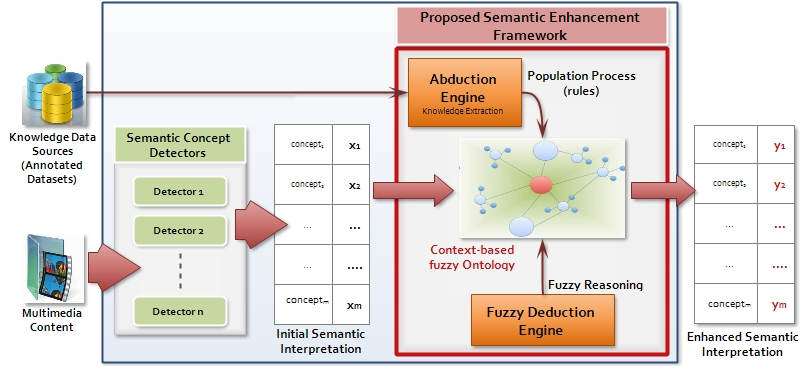
\includegraphics[width=\textwidth]{graphics/systeme}
			\caption{Proposed fuzzy context-based ontology framework for semantic Interpretation}
			\label{fig:system}
		\end{figure}

		
		\subsection{Ontology Structure}
			The objective of our proposed structure for modeling fuzzy knowledge in our ontology 
			is to handle all possible relationships that can exist between semantic concepts 
			within a defined context.

			Classical ontology description languages are not relevant to handle fuzzy knowledge.
			\emph{Fuzzy Description Logics} have been introduced by various approaches to handle 
			uncertainty and vagueness. In our work, we used the $f-\mathcal{SHIN}$ 
			\emph{Description Logics} \citep{Stoilos2005}, 
			and we used the \emph{``tableau''} algorithm \citep{Horrocks2005} for reasoning in
			$f-\mathcal{SHIN}$.  Fuzzy knowledge axioms are grouped in three parts: 
			fuzzy $ABox$ $\mathcal{A}$ for individuals, fuzzy $TBox$ $\mathcal{T}$ for concepts, 
			and fuzzy $RBox$ $\mathcal{R}$ for roles.

			Due to the large amount of multimedia content to handle, it is important to adopt a 
			modular modeling approach. Such ontology modeling has gained widespread attention. 
			Therefore, we propose to define a fuzzy ontology per a defined context.

			Let $\mathcal{K}^{f}$ be a set of fuzzy ontologies defined as follows:
			\begin{equation}
				\begin{array}{ c c l }
					\mathcal{K}^{f} & = &  \{\mathcal{K}^{f}_{t_{1}},\mathcal{K}^{f}_{t_{2}}, 
					\ldots, \mathcal{K}^{f}_{t_{n}}\} \text{ a set of $n$ fuzzy ontologies }  \\
					& &  \text{ where } \mathcal{K}^{f}_{t_{k}} \text{ is a fuzzy ontology for the context } t_{k}.
				\end{array}
			\end{equation}
			
			\begin{definition}
				A fuzzy ontology $\mathcal{K}^{f}_{t_{k}}$ of the context $t_{k}$ can be defined as follows: 

				$\mathcal{K}^{f}_{t_{k}} = \langle \mathcal{T}, \mathcal{R}, \mathcal{A} \rangle$, where
				{
					\begin{equation}
						\begin{array}{ c c l }
							\mathcal{T}  	& = 	& \{\mathsf{Shot} \sqsubseteq \top,\\
							&	& \mathsf{Concept} \sqsubseteq \top,\\
							&	& \mathsf{Context} \sqsubseteq \top,\\
							&	& \mathsf{Context}\sqsubseteq\leq{}1\mathsf{ExistsIn.Shot},\\
							&	& \mathsf{Shot}\sqsubseteq\exists\mathsf{isIndexedBy.Concept},\\
							&	& \mathsf{Concept} \sqsubseteq \exists{}\mathsf{isRelatedTo.Concept}\},\\
							\mathcal{A}	& = 	&
							\{(\langle{}\mathsf{Context},\mathsf{Shot}\rangle:\mathsf{ExistsIn})\geq
							p_{1}\\
							&	& (\langle{}\mathsf{Shot},\mathsf{Concept}\rangle:
							\mathsf{isIndexedBy}) \geq	p_{2}\\
							&	& (\langle{}\mathsf{Concept},\mathsf{Concept}\rangle:\mathsf{isRelatedTo})
							\geq p_{3}\},\\
							\mathcal{R} 	& =	& \{\mathsf{Trans(isRelatedTo)} \\
							&	& \mathsf{Disjoint(isRelatedTo,isRelatedTo^{-})}\}
						\end{array}
					\end{equation}
				}
			\end{definition}
		
		
		$\mathsf{Shot}$, $\mathsf{Context}$ and $\mathsf{Concept}$ are defined as ontology concepts.  
		The $ABox$ $\mathcal{A}$ illustrates possible relationships 
		between concepts, contexts and multimedia content shots defined in the $TBox$ $\mathcal{T}$. 
		Then, $\mathsf{isRelatedTo}$, $\mathsf{isIndexedBy}$ and $\mathsf{ExistsIn}$ 
		are defined as three roles (figure \ref{structure}).
				
		The role $\mathsf{isRelatedTo(Concept, Concept)}$ in the $\mathcal{K}^{f}_{t_{k}}$ ontology
		depicts that there is a generic relationship of a fuzzy weight $p_{3}$ between two concepts 
		within the context $t_{k}$. 
		The \revAnglais{two} roles $\mathsf{ExistsIn(Context, Shot)}$ and
		$\mathsf{isIndexedBy(Shot, Concept)}$ translate a 
		semantic interpretation for a given multimedia content shot. While the role 
		$\mathsf{ExistsIn(Context, Shot)}$ depicts that the context 
		$\mathsf{Context}$ figures in the shot $\mathsf{Shot}$ 
		with a fuzzy weight $p_{1}$, $\mathsf{isIndexedBy(Shot, Concept)}$  role
		depicts that the concept $\mathsf{Concept}$ exists in the shot $\mathsf{Shot}$ 
		with a fuzzy weight $p_{2}$.

		\begin{figure}
			\centering
			 \begin{subfigure}[b]{0.4\textwidth}
      			  	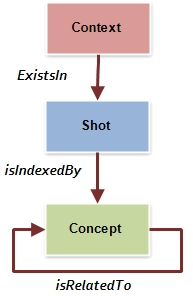
\includegraphics[scale=1]{graphics/structure2}
       				\caption{Conceptual representation of a fuzzy ontology for a given context}
       				\label{structure}
    			\end{subfigure}
			~
			\begin{subfigure}[b]{0.4\textwidth}
      			  	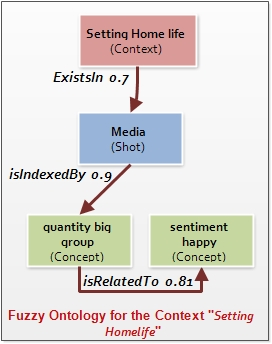
\includegraphics[scale=0.9]{graphics/example}
       				\caption{Example of the $\mathcal{K}^{f}_{Setting~Home~life}$  ontology  
			content for the context \textit{``Setting Home life''}}
       				\label{structure2}
    			\end{subfigure}
			\caption{Conceptual representation and an example of a fuzzy ontology}
		\end{figure}

		For instance, figure \ref{structure2} illustrates the ontology
		structure and individuals for the ontology $\mathcal{K}^{f}_{Setting~Home~life}$
		which is specific for the context $\mathsf{Setting~Home~life}$.
		A shot $\mathsf{Media}$ is indexed by this context with a fuzzy
		degree of $0.7$. Then, the role $\mathsf{isIndexedBy}$ $\mathsf{(Media, Quantity Big Group)}$
		depicts the fact that the shot $\mathsf{Media}$
		is indexed by the concept $\mathsf{Quantity Big Group}$ with a fuzzy
		degree of $0.9$. And finally, 
		the role $\mathsf{isRelatedTo(Quantity Big Group,Sentiment Happy)}$ 
		defines a specific relationship between concepts $\mathsf{Quantity Big Group}$ and 
		$\mathsf{Sentiment Happy}$ with a fuzzy 
		degree of $0.6$ within the ontology $\mathcal{K}^{f}_{Setting~Home~life}$. Thus, if a shot is relevant to the concept 
		$\mathsf{Quantity Big Group}$, it could be relevant too to the concept $\mathsf{Sentiment Happy}$ 
		if the context $\mathsf{Setting~Home~life}$ exists in this shot.

		As described in figure \ref{fig:system}, the proposed framework aims to handle a semantic interpretation 
		as input and to generate an enhanced one as output. Mathematically, and as input, we have a set of shots 
		where each \revAnglais{one} is tagged by some semantic concepts. And as output, the framework \revAnglais{delivers} the same 
		set of images, but with an improved concept tagging. For the ontology side, this set of shots and their 
		related concepts are translated to $Abox$ $\mathcal{A}$ within the fuzzy context-based ontology set. 
		
		\begin{definition}Let $Input$ and $Output$ be sets of quadruplet $(t_{k},c,shot_{i},(\alpha_{1}, \alpha_{2}))$. 
		Each quadruplet depicts that the shot $shot_{i}$ is tagged by the concept $c$ by a fuzzy weight 
		$\alpha_{2}$ within the context $t_{k}$, and tagged by the context $t_{k}$ by a fuzzy weight $\alpha_{1}$.
 		These quadruplets are correlated with the $\mathsf{isIndexedBy}$ and $\mathsf{ExistsIn}$ roles ($\langle(t_{k},s): 
		\mathsf{ExistsIn} \geqslant (\alpha_{1})\rangle$ and $\langle(shot_{i},c) : \mathsf{isIndexedBy} 
		\geqslant (\alpha_{2})\rangle$).
		\end{definition}
		
		\subsection{Abduction Engine and Ontology Population}

			The population process aims to extract new knowledge through an abduction engine and to populate the 
			ontology with new instances defined in a specific context, 
			as well as with their properties and relations. In what follows, we itemize the proposed abduction engine, 
			then we show how to populate the fuzzy context-based ontology with new extracted knowledge.

		\subsubsection{The Abduction Engine}

			In this section, we are particularly interested in the 
			$\mathsf{isRelatedTo}$ role (since the other two roles instances are directly populated 
			from an initial semantic interpretation).

			The key idea behind our method for the abduction engine is to explore similarities 
			between semantic concepts within an annotated multimedia content. Indeed, many annotated 
			multimedia datasets (particularly image and video content) are available and accessible:  
			\emph{ImageCLEF Flickr Photo Annotation and Retrieval} \citep{Thomee2012} and \textsc{TrecVid}  
			\citep{Over2013} training datasets, \emph{Flickr API} and \emph{Picasa API} for image/video 
			crawling, \dots are valuable data sources that can be explored in order to extract knowledge 
			to be inserted into an ontology and to be used then to enhance a semantic interpretation.


			We would like to remind that a \emph{semantic context} is an abstract meaning that cannot be well defined because 
			it makes sense only in particular situations \citep{Elleuch2011, Ksentini2012}. 
			%%%%%%%%%%%%%%%%%%%%%%%%%%%%%%%%%%%%%%%%%%%%%%%%%%%%%%%%%%%%%%%%%%%%%%%%%%%%%%%%%%%%%%
			%%%%%%%%%%%%%%%%%%%%%%%%%%%%%%%%%%%%%%%%%%%%%%%%%%%%%%%%%%%%%%%%%%%%%%%%%%%%%%%%%%%%%%
			%%%%%%%%%%%%%%%%%%%%%%%%%%%%%%%%%%%%%%%%%%%%%%%%%%%%%%%%%%%%%%%%%%%%%%%%%%%%%%%%%%%%%%
			For example, the concept \emph{``airplane\_{}flying''} is considered as
			a context since it specifies a particular relationship between two other
			concepts: \emph{``sky'''} and \emph{``airplane''}. 

			%%%%%%%%%%%%%%%%%%%%%%%%%%%%%%%%%%%%%%%%%%%%%%%%%%%%%%%%%%%%%%%%%%%%%%%%%%%%%%%%%%%%%%
			%%%%%%%%%%%%%%%%%%%%%%%%%%%%%%%%%%%%%%%%%%%%%%%%%%%%%%%%%%%%%%%%%%%%%%%%%%%%%%%%%%%%%%
			%%%%%%%%%%%%%%%%%%%%%%%%%%%%%%%%%%%%%%%%%%%%%%%%%%%%%%%%%%%%%%%%%%%%%%%%%%%%%%%%%%%%%%
			In our case, we define a context as follows:
			\begin{definition} 
				A context is defined as a concept that can stipulate a specific relationship 
				between other concepts.
			\end{definition}

			Thanks to such a definition, we can give a more abstract meaning of a context rather than a \revAnglais{spatial} or 
			temporal information \citep{Brilhault2009}, and also provide an automated way to discover contexts 
			within a concept set.
                	Then, for a given concept $c$, we look for some eventual similarities
			between other concepts within shots annotated with the concept $c$. 
			If such relationships are found, the concept $c$ is considered as a context.

			We use the vector space model based method to compute the similarity between concepts.
			\begin{equation}
				sim(c,d) = cossim(c,d) = \frac{\vec{V_{c}} . 
				\vec{V_{d}}}{|V_{c}| . |V_{d}|}
			\end{equation}
			where for each concept $c$, a weighted vector $V_{c}$ can be constructed as
			\begin{equation}
			V_{c} =\{v^{shot_{1}}_{c},v^{shot_{2}}_{c}, \dots, v^{shot_{m}}_{c}\}
			\end{equation}
			where $v^{shot_{i}}_{c} \in [0,1]$ is the weight of the concept $c$ in the video 
			shot $shot_{i}$, and 
			\begin{equation}
				v_{i}= tf_{shot_{i},c}.idf_{c} = tf_{shot_{i},c}.log\frac{|S|}{|s_{c}|}
			\end{equation}
			where $tf_{shot_{i},c}$ is the frequency of the concept $c$ in the
			video shot $shot_{i}$, $|S|$ is the total number of shots and $|s_{c}|$ is 
			the number of shots tagged by the concept $c$.


			Based on what has just been developed, we propose a formal method to discover contexts. 
			%In our case, we populate a fuzzy ontology $\mathcal{K}^{f}_{t_{k}}$ of the context $t_{k}$ as follows:
			%%%%%%%%%%%%%%%%%%%%%%%%%%%%%%%%%%%%%%%%%%%%%%%%%%%%%%%%%%%%%%%%%%%%%%%%%%%%%%%%%%%%%%
			%%%%%%%%%%%%%%%%%%%%%%%%%%%%%%%%%%%%%%%%%%%%%%%%%%%%%%%%%%%%%%%%%%%%%%%%%%%%%%%%%%%%%%
			%%%%%%%%%%%%%%%%%%%%%%%%%%%%%%%%%%%%%%%%%%%%%%%%%%%%%%%%%%%%%%%%%%%%%%%%%%%%%%%%%%%%%%			
			Thus, we define the similarity $sim_{t_{k}}(c, d)$ as a similarity measurement between the 
			two concepts 
			$c$ and $d$ within the context $t_{k}$. This similarity will be used as a fuzzy degree 
			for the rule that relates the concepts $c$ to the concept $d$ within the role 
			$\mathsf{isRelatedTo}$ for the $\mathcal{K}^{f}_{t_{k}}$ ontology.


			Furthermore, $\mathsf{isRelatedTo}$ is a \revAnglais{non-symmetric}  role
			(as appears in the \emph{Rbox} $\mathcal{R}$). 
			As an example, when talking about the concept \emph{``car\_racing''}, 
			it is obvious that we talk about the concept \emph{``car''}, but  the \revAnglais{opposite}
			in not often true. Thus $sim(car,car\_racing) \neq sim(car\_racing ,car)$.
			To do that, the similarity function that is used to compute the similarity $sim_{t_{k}}(c, d)$ 
			in a defined context  $t_{k}$ has to be \revAnglais{non-symmetric}. 
			Then, the two vectors $V_{c}$ and $V_{d}$ are modified as follow to ensure that  
			$sim_{t_{k}}(c, d) \neq sim_{t_{k}}(d, c)$:

		
		\begin{equation}
			\begin{array}{ c c l }
			V_{c} & = & \{v^{shot_{1}}_{c},v^{shot_{2}}_{c}, \dots, v^{shot_{m}}_{c}\}\\
			%%%%%%%%%%%%%%%%%%%%%%%%%%%%%%%%%%%%%%%%%%%%%%%%%%%%%%%%%%%%%%%%%%%%%%%%%%%%%%%%%%%%%%
			%%%%%%%%%%%%%%%%%%%%%%%%%%%%%%%%%%%%%%%%%%%%%%%%%%%%%%%%%%%%%%%%%%%%%%%%%%%%%%%%%%%%%%
			%%%%%%%%%%%%%%%%%%%%%%%%%%%%%%%%%%%%%%%%%%%%%%%%%%%%%%%%%%%%%%%%%%%%%%%%%%%%%%%%%%%%%%			
			%V_{d} & = & 
			V_{d} & = & 
			%%%%%%%%%%%%%%%%%%%%%%%%%%%%%%%%%%%%%%%%%%%%%%%%%%%%%%%%%%%%%%%%%%%%%%%%%%%%%%%%%%%%%%
			%%%%%%%%%%%%%%%%%%%%%%%%%%%%%%%%%%%%%%%%%%%%%%%%%%%%%%%%%%%%%%%%%%%%%%%%%%%%%%%%%%%%%%
			%%%%%%%%%%%%%%%%%%%%%%%%%%%%%%%%%%%%%%%%%%%%%%%%%%%%%%%%%%%%%%%%%%%%%%%%%%%%%%%%%%%%%%			
			\{v^{shot_{1}}_{d},v^{shot_{2}}_{d}, \dots, v^{shot_{m}}_{d}\}\\
			& & \text{ where for every considered shot } shot_{i} \text{ in both } V_{c} \text{ and } V_{d},\\
			& &  \text{we have } v^{shot_{i}}_{c}\neq 0 \text{ and } v^{shot_{i}}_{t_{k}} \geqslant \gamma
			\end{array}
		\end{equation}
		
		we suggest $\gamma \in [0,1]$  as a threshold to judge if a concept is strongly relevant 
		to a video shot or not. Thus, only tagged shots by the concept $c$ and that are strongly 
		tagged by the concept/context $t_{k}$ are considered for both $V_{c}$ and $V_{d}$ in order to guarantee 
		the \revAnglais{non-symmetric} aspect of the role $\mathsf{isRelatedTo}$.


		\subsubsection{Ontology Population}	
		\label{pop1}
		The ontology population  passes through two steps: 
		\begin{enumerate}
			\item \textit{\revAnglais{Knowledge} Population}: For each defined context $t_{k}$, 
			this step constructs an empty ontology $\mathcal{K}^{f}_{t_{k}}$ based on the proposed structure detailed in 
			the previous section. Then, the context $t_{k}$ is instantiated as an individual
			from the class $\mathsf{Context}$. Next, for every new similarity 
			$sim_{t_{k}}(c, d)$ computed between two concepts $c$ and $d$ within the 
			context $t_{k}$, two new instantiations from the class $\mathsf{Concept}$ 
			are introduced in the ontology for both concepts $c$ and $d$, and finally  
			a new $\mathsf{isRelatedTo}$ role instantiation between $c$ and $d$  
			is inserted to the $\mathcal{K}^{f}_{t_{k}}$ ontology with a fuzzy weight
			equal to this similarity value.
 
			\item \textit{Semantic Interpretation Population}
			In this step, semantic interpretations about shots 
			are introduced to the set of fuzzy ontologies $\mathcal{K}^{f}$. 
			For a given shot $shot_{i}$, and for each context $t_{k}$, if $shot_{i}$ 
			is tagged by the context $t_{k}$, then:
				\begin{enumerate}
					\item the shot $shot_{i}$ is instantiated as an individual from 
					the class $\mathsf{Shot}$,
					\item a new instantiation of the role $\mathsf{ExistsIn}$ is introduced 
					between $shot_{i}$ and $t_{k}$ within the ontology $\mathcal{K}^{f}_{t_{k}}$,
					\item for every concept $c$ that tags $shot_{i}$, $c$ is introduced to the 
					ontology $\mathcal{K}^{f}_{t_{k}}$ as an individual from the class 
					$\mathsf{Concept}$, and a new $\mathsf{IsIndexedBy}$ role \revAnglais{instantiation}
					is created between $shot_{i}$ and $c$.
				\end{enumerate}
		\end{enumerate}

		Once the two steps are performed, a set of fuzzy context-based ontology \revAnglais{is} built and 
		ready to fire the reasoning engine (the deduction engine) in order to
		generate an enhanced semantic interpretation.
		
		\subsection{Ontology Reasoning}
		Within the scope of reasoning in this paper, we are particularly interested in the outputs that
		such a system produces. In such a case, and for each ontology $\mathcal{K}^{f}_{t_{k}}$ 
		of the context $t_{k}$, we generate 
		the corresponding ontology $\mathcal{K'}^{f}_{t_{k}}$ as an ontology that handle enhanced 
		semantic interpretations. This is done by 
		interpreting the $Abox$ $\mathcal{A}$ in order to look for updated or additional relationships between 
		$\mathsf{Shot}$ and $\mathsf{Concept}$ (for the role name
		$\mathsf{isIndexedBy}$).

		We used and adapted the \emph{``tableau''} based reasoning algorithm \citep{Dentler2011}. The latter  
		adopts a federated reasoning process with our set of fuzzy ontologies. Thus, each fuzzy ontology is 
		associated with a local reasoner. The final and global reasoning  result is inferred through 
		all the local reasoner results. 


		Considering concepts and roles as fuzzy sets, the semantics of concepts and roles are defined 
		by fuzzy interpretations $\mathcal{I} = \langle{}\triangle^{\mathcal{I}}= , \cdot^{\mathcal{I}}\rangle{}$, 
		where $\triangle^{\mathcal{I}}$ is a nonempty domain, and $\cdot^{\mathcal{I}}$ is an interpretation 
		function mapping individuals $a$ into $a^{\mathcal{I}} \in \triangle^{\mathcal{I}}$,
		and mapping concept (roles) names $A(R)$ into membership functions 
		$A^{\mathcal{I}}(R^{\mathcal{I}}) : \triangle^{\mathcal{I}} (\triangle^{\mathcal{I}} * \triangle^{\mathcal{I}} ) 
		\rightarrow [0, 1]$. 
		An interpretation $\mathcal{I}$ satisfies a knowledge database $\mathcal{K}^{f}_{}$, 
		if and only if  $\mathcal{I}$ satisfies any
		axiom in $\mathcal{R}$, $\mathcal{T}$ and $\mathcal{A}$. $\mathcal{K}^{f}_{}$ is satisfiable 
		if and only if it has a fuzzy model.

		We define the symbols  $\rhd$ and  $\lhd$ as a placeholder for the  inequalities 
		($\leq$, $<$, $\geq$ and $>$) and the symbol $\bowtie$ as a placeholder for all types of inequalities.
		
		\begin{definition}
			let $R_{A}$ be the set of roles occurring in $\mathcal{A}$, $I_{\mathcal{A}}$ the set 
			of individuals in $\mathcal{A}$ and $\mathcal{X} = \{\leq, <, \geq, >\}$. A fuzzy tableau 
			$T$ for $\mathcal{A} ~ w.r.t ~ \mathcal{R}$ is a quadruple
			$(S, \mathcal{L, E, V})$ in such a way that:
			\begin{itemize}
				\item $S$ is a nonempty set of individuals (considered also as nodes),
				\item $\mathcal{L} : S \longrightarrow 2^{sub(A)} \times \mathcal{X} \times [0,1]$ 
					maps each individual in $S$ to membership triples,
				\item $\mathcal{E} : R_{A} \longrightarrow 2^{S \times S} \times \mathcal{X} \times [0,1]$ 
					maps each role to membership triples,
				\item $\mathcal{V} : I_{\mathcal{A}} \longrightarrow S$ maps individuals occurring in 
					$\mathcal{A}$ to elements in $S$.
			\end{itemize}
		For all	$s,t \in S$, $R\in R_ {A}$ and $C,E \in sub(\mathcal{A})$, $T$ satisfies a particular 
		transformation rule defined in algorithm \ref{algo1}	
		(in addition to default transformation rules defined in \citep{Stoilos2005}).	

		\begin{algorithm}
				\If	{ $\langle(t_{k},shot_{i}) : \mathsf{ExistsIn} \bowtie \alpha_{1}\rangle 
					\in \mathcal{A}$ AND \\
					$\langle(shot_{i},c) : \mathsf{isIndexedBy} \bowtie \alpha_{2}\rangle \in \mathcal{A}$ 
					AND \\
					$\langle(c,d) : \mathsf{isRelatedTo} \bowtie \alpha_{3}\rangle \in \mathcal{A}$}
					{
					 \lIf	{$\langle(shot_{i},d) : \mathsf{isIndexedBy} \bowtie 
						\alpha_{4}\rangle \notin \mathcal{A}$} 
						{\\$\mathcal{A'} := \mathcal{A} \sqcup \{ \langle{}\mathsf{shot_{i}},
							\mathsf{d}\rangle:
							\mathsf{isIndexedBy}) \bowtie \alpha_{4}\}$\\
							and $\langle \langle\mathcal{V}(shot_{i}),\mathcal{V}(d)\rangle
							\bowtie \alpha_{4}\rangle 
							\in \mathcal{E}(\mathsf{isIndexedBy})$ \\
							where $\alpha_{4} = \alpha_{1} \times \alpha_{2} \times \alpha_{3}$}
						\lElse{$\langle \langle\mathcal{V}(shot_{i}),\mathcal{V}(d)\rangle
							\bowtie \alpha_{4}'\rangle 
							\in \mathcal{E}(\mathsf{isIndexedBy})$ \\
							where $\alpha_{4}' = max(\alpha_{4}, (\alpha_{1} \times \alpha_{2}
							\times \alpha_{3}))$}}
					\caption{Transformation Rule: Property 1}
					\label{algo1}
				\end{algorithm}
				
		\end{definition}
		Property 1 is a consequence of the fact that if there are three \revAnglais{axioms} in $\mathcal{A}$ 
		where $shot_{i}$ is indexed by a concept $c$, and the context $t_{k}$ exists in the $shot_{i}$, 
		then the $shot_{i}$ could be indexed by the concept $d$ taking into account that within the 
		fuzzy ontology of the context $t_{k}$, there is a relationship between the two concepts $c$ and $d$.
		If this new deduced relationship already exists in the ontology, then we only update its fuzzy weight.

		We used and adapted a \emph{“tableau”} based reasoning algorithm.
 		For a given context-based ontology, the latter model the knowledge in form of 
		a tree in which nodes correspond to individuals (semantic concepts, semantic contexts and shots) 
 		and edges correspond to the defined roles ($\mathsf{isIndexedBy}$,$\mathsf{isRelatedTo}$,
 		and $\mathsf{ExistsIn}$).
 		Each node $x$ is labeled with a set of concepts $\mathsf{L}(x)$ that the
 		individual must satisfy, and each edge is labeled with a role name.
 		The reasoning algorithm starts with a single node labeled $\{D\}$ (in our case, a
 		node labeled as a shot), and proceeds by repeatedly applying a set of expansion 
		rules that recursively decompose the concepts in node labels.

		The reasoning process should not be endless. This problem can \revAnglais{deal} with the use 
		of a blocking technique: stopping the expansion when a cycle is detected. The 
		blocking procedure consists in checking the label of each new node $y$, and if 
		it's a subset of the label of an existing node $x$, then the expansion of $y$ 
		is stopped: $x$ is said to block $y$.
		
		Thus, the reasoning process termination is \revAnglais{guaranteed}: all concepts in node labels
		are derived from the decomposition of $D$, so all node labels must be a subset  
		of the sub-concepts of $D$. A cycle should be avoided within a finite number of expansion steps.

		%%%%%%%%%%%%%%%%%%%%%%%%%%%%%%%%%%%%%%%%%%%%%%%%%%%%%%%%%%%%%%%%%%%%%%%%%%%%%%%%%%%%%%%%%%%%%%%%%%
		%%%%%%%%%%%%%%%%%%%%%%%%%%%%%%%%%%%%%%%%%%%%%%%%%%%%%%%%%%%%%%%%%%%%%%%%%%%%%%%%%%%%%%%%%%%%%%%%%%
		\begin{algorithm}
			
			\SetAlgoLined
			%\KwData{$Input \neq \emptyset$ and $Output = \emptyset$ }
			%\KwResult{$Output \neq \emptyset$ }
			\For{each shot \textbf{$shot_{i} \in \mathsf{Shot}$}}{
				\For{each concept \textbf{$c$} connected with the shot 
				\textbf{$shot_{i}$} by an $\mathsf{isIndexedBy}$ labeled edge}{
					Handle\_isRelatedTo\_Role($shot_{i}$,$c$);
				}
			}
			\caption{Reasoning Process for enhancing a semantic interpretation about shots.}
			\label{algo112}
		\end{algorithm}
		
		%%%%%%%%%%%%%%%%%%%%%%%%%%%%%%%%%%%%%%%%%%%%%%%%%%%%%%%%%%%%%%%%%%%%%%%%%%%%%%%%%%%%%%%%%%%%%%%%%%
		%%%%%%%%%%%%%%%%%%%%%%%%%%%%%%%%%%%%%%%%%%%%%%%%%%%%%%%%%%%%%%%%%%%%%%%%%%%%%%%%%%%%%%%%%%%%%%%%%%
		
		\begin{algorithm}
			
			\SetAlgoLined
			%\KwData{$Input \neq \emptyset$ and $Output = \emptyset$ }
			%\KwResult{$Output \neq \emptyset$ }
			\textbf{Function} Handle\_isRelatedTo\_Role($shot_{i}$,$c$)\\
			  \eIf{isMarked($c$)}{
			  return\;}
			  {
			  		\For{each concept $d$ connected with $c$ by an edge labeled
			  		$\mathsf{isRelatedTo}$}{Mark($c$)\;
					apply Algorithm \ref{algo1} \;
					Handle\_isRelatedTo\_Role($shot_{i}$,$d$)\;
				}	
			}
			\caption{Recursive call for \emph{``Handle\_isRelatedTo\_Role()''} Function}
			\label{algo111}
		\end{algorithm}
		%%%%%%%%%%%%%%%%%%%%%%%%%%%%%%%%%%%%%%%%%%%%%%%%%%%%%%%%%%%%%%%%%%%%%%%%%%%%%%%%%%%%%%%%%%%%%%%%%%
		%%%%%%%%%%%%%%%%%%%%%%%%%%%%%%%%%%%%%%%%%%%%%%%%%%%%%%%%%%%%%%%%%%%%%%%%%%%%%%%%%%%%%%%%%%%%%%%%%%

		The $\mathsf{isRelatedTo}$ role is cyclic and transitive. Such a
		definition \revAnglais{makes} the termination and the decidability of our reasoning process hard. We adapted 
		the \emph{``tableau''} algorithm is such a way to  solve this problem. 
		Apart from the generic blocking technique above detailed, we used a second 
		blocking technique which marks every passage through  
		semantic concepts that are connected with $\mathsf{isRelatedTo}$ role labeled
		edges. We used two functions: $Mark(c)$ which marks a concept $c$, and
 		$isMark(c)$ which returns whether the concept $c$ is marked or not yet.

		Algorithms \ref{algo112} and \ref{algo111} detail how we extend a semantic interpretation of a given
 		shot taking into consideration the proposed blocking technique. 

		The node marking test in the algorithm \ref{algo111} allows to detect an
 		eventual cycle. Then, a possible endless call to the
 		\emph{``Handle\_isRelatedTo\_Role()''} recursive function is blocked. 
		The proposed algorithm achieved the decidability of our reasoning process.

		\subsection{Ontology Evolving}
		\label{section:evolving}
		Evolving and updating fuzzy knowledge is a task that must be addressed in an ontology life cycle. 
		Such a test consists in updating the ontology content in order to take into account both, eventual erroneous 
		or senseless knowledge, or newer knowledge. In our work, we consider the evolution of ontology individuals content 
		and not the conceptual level. Then, only individuals and \revAnglais{inter-relationships} in $Abox$ $\mathcal{A}$ 
		could be updated.

		The evolving task proceeds as follows: Let $\mathcal{A}$ be the $ABox$ of an ontology, and $\mathcal{A_{+}}$ 
		the updated one. %, and $\mathcal{A'}$ the final considered knowledge after the evolving process.
 		Then the evolving task can be illustrated with the algorithm \ref{algo3}. The latter always \revAnglais{considers}
		the new discovered knowledge by updating the fuzzy weight of a $\mathsf{isRelatedTo}$ 
		role to the new value defined in $\mathcal{A_{+}}$.
		
		\begin{algorithm}
				
				\If	{$\langle(c,d) : \mathsf{isRelatedTo} \bowtie \alpha \rangle \in \mathcal{A}$ AND \\
					 $\langle(c,d) : \mathsf{isRelatedTo} \bowtie \alpha'\rangle \in \mathcal{A_{+}}$ }
					{
					 $\mathcal{A} := \mathcal{A}  \diagdown \{
					 \langle{}(\mathsf{c},\mathsf{d}):
							\mathsf{isRelatedTo}\rangle{} \bowtie \alpha\}$\\
					$\mathcal{A} := \mathcal{A} \sqcup \{ \langle{}(\mathsf{c},\mathsf{d}):
							\mathsf{isRelatedTo}\rangle{} \bowtie \alpha'\}$\\
					}
				\caption{The knowledge evolving task}
				\label{algo3}
		\end{algorithm}

		In what follows, we show how to generate the new $ABox$ $\mathcal{A_{+}}$ used to update the ontology content. 
		Thus, we consider that the defined fuzzy ontologies are populated through
		a knowledge discovery technique based 
		on annotation data. We consider, too, that this extracted knowledge may
 		be inaccurate depending on many factors (annotators quality, dataset content quality, \dots). 
		Then, we propose  to correct the ontology contents 
		through inspecting $\mathsf{isRelatedTo}$ roles by human experts. 

		We thus propose a user interface to let the experts give their relevance judgment for a given role within a given 			contextual ontology. For a given context $t_{k}$ and an affiliated $\{ \langle{}(\mathsf{c},\mathsf{d}): 
		\mathsf{isRelatedTo}\rangle{} \bowtie \alpha\}$ role, this user interface shows
 		to the expert a set of rows where each one details one shot that both the context 
		$t_{k}$ and the concept $c$ exist. The expert then has to select one from these four options:
		\begin{itemize}
			\item $Strongly~Relevant$ when the concept $d$ effectively in the showed shot. We 
				consider that the fuzzy weight for this case is higher or equal to $0.7$,
			\item $Weakly~Relevant$ When the concept $d$ may \revAnglais{exist} in the showed shot. We 
				consider that the fuzzy weight for this case is higher or equal to $0.3$ 
				and lower than $0.7$,
			\item $Not~Relevant$ When the concept $d$ does not exist in the showed shot. We 
				consider that the fuzzy weight for this case is lower than $0.3$,
			\item $Skip$ when the expert \revAnglais{cannot} judge clearly if the concept $d$ 
				exists or not in the showed shot.
		\end{itemize} 
		
		The original value of a fuzzy weight of a given role is taken into
		consideration and appears when the evolving user interface displays a role to 
		an expert. In fact, every role is displayed 
		with its fuzzy weight, and the expert \revAnglais{judges} to input his judgment (if he
		\revAnglais{finds} that the role is not pertinent) or to skip to analyze another role.
		
		After the evaluation process done by the experts, the \revAnglais{knowledge} evolving task computes new fuzzy 
		weights for evaluated roles. These weights are computed as follows:
		Let $N_{experts}$ be the number of experts who evaluated the role $r$. Let $N_{StrongR}$, 
		$N_{WeakR}$ and $N_{NotR}$ be, respectively, the number of $Strongly~Relevant$, $Weakly~Relevant$ 
		and $Not~Relevant$ judgments made by the $N_{experts}$ experts for the role $r$ where:
		\begin{equation}
			N_{experts} \geqslant  N_{StrongR} +  N_{WeakR} +  N_{NotR}.
		\end{equation}

		Then, we compute the new fuzzy weight for the evaluated role $r$ as follows:
		
		\begin{equation}
		\alpha'=\left\{
			\begin{array}{l c}
				max(\alpha, \frac{N_{StrongR}}{N_{experts}})	& 
					\text{\scriptsize{if $N_{StrongR} \geqslant (N_{WeakR},N_{NotR})$}} \\
				min(\alpha, \frac{1-N_{WeakR}}{N_{experts}}) & 
					\text{\scriptsize{if $N_{WeakR} > (N_{StrongR},N_{NotR})$}}\\
				min(\alpha, \frac{1-N_{NotR}}{N_{experts}})  &
					\text{\scriptsize{if $N_{NotR} > (N_{StrongR},N_{WeakR})$}}
			\end{array}
		  \right.
		\end{equation}

		The equation above is inspired by the majority vote. The new computed role 
		fuzzy weight is based on whether experts are commonly improving or disregarding a role.
		
		For an analyzed role, only one new fuzzy weight will be considered
		and introduced to the ontology. Thus, no eventual conflicting situation 
		occurs when firing the reasoning engine.
		This choice is preselected by the initial value of fuzzy role weight.

		\subsection{Approach Scalability}

		The scalability aspect is very important and concerns mainly two aspects: 
		how our framework \revAnglais{performs} when a large amount of concepts 
		and interrelationships are defined, and when the number of contexts increases. 

		Our proposed approach could be considered as scalable:
		at first, the $Tbox$ $\mathcal{T}$ remains unchanged, and only new $Abox$ $\mathcal{A}$ 
		instances are \revAnglais{being} handled within the defined contextual ontologies. Then, the amount of knowledge 
		populated within an ontology depends only on what has been gathered from annotated 
		video datasets in addition to the semantic interpretation of the analyzed video shot. 
		Secondly, since the proposed approach is decomposed into several ontologies, 
		the deduction engine is applied only on $Abox$ $\mathcal{A}$ that are related only to each defined contexts. 
		This leads to an optimized and a lightened reasoning process: only partial 
		defined roles in ontologies will be considered and fired.
		
		In the next section, we conduct an experiment to investigate our approach effectiveness and scalability.
		

		
	%%%%%%%%%%%%%%%%%%%%%%%%%%%%%%%%%%%%%%%%%%%%%%%%%%%%%%%%%%%%%%%%%%%%%%%%%%%%%%%%%%%%%%%%%%
	%%%%%%% EVALUATION
	\section{Experimental Study}
		\label{c2_3}
		In the previous chapter, we discussed our participation within \revAnglais{the} \textsc{TrecVid 2010}. 
		Only the deduction process was taken into consideration since we used a manually predefined 
		set of rules, and  we were interested in visual (key frames) semantic analysis. 
		
		In order to illustrate the semantic enhancement of concept detection introduced 
		by our proposed ontology-based framework, we have conducted an experiment within a 
		different multimedia evaluation campaign. Hence, we expose the experimental setup and the 
		obtained results of our framework within \textit{ImageClef 2012} \citep{Thomee2012}
		at the \textit{Photo Annotation and Retrieval} Task. 
		Finally, we discuss the scalability of our proposed framework.


		\subsection{Datasets Description}

		The \textit{ImageClef 2012} Photo Annotation and Retrieval task provides a dataset built from
		Flickr social shared photos. This image dataset consists of 25 thousand images:
		15 thousand for the learning process and 10 thousand for the test one. In addition
		to the images, 94 semantic concepts are defined referring to many and various 
		subjects (people, nature, events, \dots). 

		\subsection{Evaluation metrics}
		In order to be able to compare different indexing approaches, various system 
		effectiveness metrics have been used. These metrics are commonly based on precision
		(which is defined as the number of relevant answers as a part of the total number
		of retrieved ones), and recall (which is defined as the number of relevant answers
		as part of total relevant ones in the collection). In our experiments, we consider the two
 		evaluation measures: \emph{Interpolated Mean Average Precision} (\textit{$map_{i}$}) and \emph{Interpolated 
		Geometric Mean Average Precision} (\textit{$gmap_{i}$}) \citep{Thomee2012}
		for \revAnglais{the} \textit{ImageClef 2012} Flickr Photo Annotation and Retrieval task.

		The \textit{$gmap_{i}$} is considered as an extension to the \textit{$map_{i}$} measure as it uses the same 
		computing procedure, but it's very useful when focusing on low performing semantic 
		interpretation for particular concepts

		
			\subsection{Experiments with \textit{ImageClef 2012} dataset}
		
		With this experiment, we aim to explore all the 15 thousand annotated images in order 
		to extract valuable fuzzy \revAnglais{Knowledge}. The latter will be used then within the deduction engine 
		to evaluate the knowledge-based semantic enhancement performances. The obtained results will be compared 
		to a \revAnglais{non-knowledge-based} concept detection approach detailed in \citep{Ksibi2012}. Thus, we
		used the results given by the \revAnglais{non-knowledge-based} method as input for our framework looking 
		for enhancing the semantic interpretation and for proving the effectiveness of the use of
		fuzzy context-based ontology and fuzzy reasoning in multimedia retrieval
		systems.

			\subsubsection{The abduction process}
		In the interest of populating our proposed ontology, we start by defining the set of considered contexts. 
		At first, we consider every concept as a context, and then, we look for specific relationships between other 
		concepts within this context. If any relationships are found, the defined concept will be considered
		as a context, else, the concept will not be considered as a context.
		By doing so, our proposed framework can provide automatically a set of context to work with. We consider 
		that a context exists in a shot only if this latter is strongly tagged by that context to a degree equal 
		to or higher than $0.7$. Then, we adjust the value of the threshold $\gamma$ at $0.7$.

		Our experimentation has led to define 90 contexts among the defined 94 concepts in \textit{ImageClef 2012} dataset. 
		Table \ref{table:context-based_ontology} enumerates a partial view of this set of contexts, 
		and shows the first and the last 5 contexts sorted 
		by the number of extracted $\mathsf{isRelatedTo}$ roles.
		%with a fuzzy weight equal to or higher than $0.5$.
		\begin{table*}
			\centering	
			\caption{Distribution of extracted $\mathsf{isRelatedTo}$ roles according to 
			their fuzzy weights and the defined context}
			\label{table:context-based_ontology}
				\begin{tabular}{c l c c c c c c c c c c} \hline
				~&\multirow{3}{*}{\textbf{Detected Contexts}}& \multicolumn{4}{c}{\scriptsize 
						\textbf{Number of extracted fuzzy rules according}}\\
				~& & \multicolumn{4}{c}{\scriptsize  \textbf{to their fuzzy weight intervals}}\\ 		
				~& & \small{$[0, 0.3[$} & \small{$[0.3, 0.5[$} & \small{$[0.5, 0.7[$} & 
				\small{$[0.7, 1.0]$} \\ 		\hline \hline
			\scriptsize{1}&\small{sentiment\_euphoric}	&783	&605	&510	&534\\
			\scriptsize{2}&\small{sentiment\_happy}		&2020	&864	&519	&444\\
			\scriptsize{3}&\small{setting\_sportsrecreation}&1264	&752	&483	&456\\ 
			\scriptsize{4}&\small{age\_child}		&1045	&649	&493	&441\\ 
			\scriptsize{5}&\small{relation\_familyfriends}	&1150	&903	&398	&522\\ \hline
			\scriptsize{86}&\small{fauna\_cat}		&115	&105	&91	&203\\ 
			\scriptsize{87}&\small{fauna\_insect}		&107	&63	&43	&192\\
			\scriptsize{88}&\small{fauna\_rodent}		&43	&53	&43	&139\\ 
			\scriptsize{89}&\small{fauna\_amphibianreptile}	&24	&29	&43	&127\\ 
			\scriptsize{90}&\small{fauna\_spider}		&3	&20	&16	&48\\ \hline \hline
			\multicolumn{2}{c}{\textbf{All contexts}}	&91803 	&50210	&27435	&33667\\
			 \hline \hline
			\multicolumn{2}{c}{\textbf{Total}}& \multicolumn{4}{c}{\textbf{203115 $\mathsf{isRelatedTo}$ 
								roles}}\\ \hline
			\end{tabular}
		\end{table*}
		

		Taking some roles as examples, we focus on the contexts \emph{age\_adult}, \emph{transport\_car},
		\emph{setting\_homelife} and \emph{age\_teenager}:
		\begin{equation*}
			\begin{array}{ c c l l}
			R1 & - &\mathsf{isRelatedTo}_{age\_adult} 
				& (age\_teenager,sentiment\_scary) \geq 0.12\\
			R2 & - &\mathsf{isRelatedTo}_{transport\_car}
				& (sentiment\_happy,timeofday\_day) \geq 0.95\\
			R3 & - &\mathsf{isRelatedTo}_{setting\_homelife} 
				& (quantity\_biggroup,sentiment\_happy) \geq 0.81\\
			R4 & - &\mathsf{isRelatedTo}_{age\_teenager}
				& (sentiment\_funny,quantity\_two) \geq 0.48
			
			\end{array}
		\end{equation*}

		The role $R1$ depicts that in the case of a shot tagged by the concept \emph{age\_teenager} 
		and strongly tagged by the concept \emph{age\_adult} (here considered as a context), then the concept 
		\emph{sentiment\_scary} could exist in the same shot. Naturally, this case is not always true, 
		and this is why the fuzzy weight of this role is very weak ($0.12$).
		Then, the roles $R2$  and $R3$ depict strong relationships between the two concepts 
		\emph{sentiment\_happy} and \emph{timeofday\_day} within the context \emph{transport\_car},
		and between the two concepts \emph{quantity\_ biggroup} and \emph{sentiment\_happy} within 
		the context \emph{setting\_homelife}. These two relationships are considered as strong roles 
		(where the fuzzy weights are high).

		Finally, and after extracting knowledge from the learning dataset and generating $\mathsf{isRelatedTo}$
		roles, these roles are introduced into the corresponding fuzzy context based ontology (as detailed in section \ref{pop1}).
		
		We continue to experiment deduction engine as a fuzzy reasoning process based 
		on these roles to assess the semantic enrichment in the next section.

		\subsection{Enhancement Evaluation}
		To evaluate our proposed framework, we have compared our results with an image annotation 
		method detailed in \citep{Ksibi2012} within the \emph{Flickr Photo Annotation Task}. 
		The latter is based on constructing a semantic context network to depict intrinsic 
		contextual information between concepts in order to enhance automatic photo annotation performances.
		In our work, we are interested in improving this method. Thus, we used the results given by this 
		method as input to our framework aiming at enhancing the semantic interpretation.


		Considering constructed fuzzy context-based ontology set in the previous section, 
		we introduce the $Input$ set  to these ontologies. Then, the deduction engine is fired. 
		Finally, the $Output$ set is extracted and translated into a semantic interpretation as an 
		enhanced one. For the deduction engine, only 
		$\mathsf{isRelatedTo}$ roles with a fuzzy weight higher or equal to $0,7$ are addressed. 
		We think that the other roles figure weak fuzzy weights and shouldn't be used in the deduction process.
		
		After extracting the $Output$ set, the system is ready for evaluation. So, we used 
		the evaluation tool supplied by \emph{ImageCLEF} 
		(\emph{imageclef2012CR}). We carried out unit evaluations over ontologies 
		(each ontology is evaluated separately). Finally, we applied an overall assessment showing 
		the performance of our framework (all ontologies combined). 

		Table \ref{overall} displays enhancement performances delivered by our proposed framework over 
		the \revAnglais{non-knowledge-based} approach detailed in \citep{Ksibi2012}. Table \ref{unit} shows enhancement 
		performances delivered by each defined fuzzy context-based ontology.
				

		In order to make table \ref{overall} and table \ref{unit} interpretation easier, three styles 
		were used: bold values depict enhancing performances compared to the corresponding 
		evaluation of the system detailed in \citep{Ksibi2012}, underlined values depict a 
		decreasing performance, and finally, the \revAnglais{non-styled} values depict same performance 
		as reference. 

		\begin{table*}[ht!]
			\centering	
			\caption{\textsc{ImageClef 2012}: Overall performance evaluation}
			\label{overall}
		\begin{tabular}{p{6cm}|c|c|c|c} 
			&
			\multicolumn{2}{c|}{\textbf{\textit{map$_{i}$}}} &
			\multicolumn{2}{c}{\textbf{\textit{gmap$_{i}$}}}  \\
			& \textit{Value} & \textit{Enhancement} & \textit{Value} & \textit{Enhancement}  \\
			\hline  
			Our proposed framework  & 
						\textbf{0,1324} & $5.08 \% $ & 
						\textbf{0, 0807} & $3.46 \% $ \\
			System in \cite{Ksibi2012}   & $0.126$ & - & $0.078$  \\
			\hline 
		\end{tabular}
		\end{table*}


\begin{table*}[ht!]
	\centering
	\caption{\textsc{ImageClef 2012}: Unit performances evaluation}
	\label{unit}
\begin{scriptsize}
\begin{tabular}{|c|lcc||c|lcc|}
	\hline
	\#  &\textbf{\textit{Context}}	& \multicolumn{2}{l||}{\textbf{\textit{{~~~~Evaluation} }}}
	&
	\# 		& 
	\textbf{\textit{Context}} 	& 
	\multicolumn{2}{l|}{\textbf{\textit{{~~~~Evaluation} }}} \\
	%\hline
	%#
        	&  &  \textbf{map$_{i}$} &  \textbf{gmap$_{i}$} &   & & \textbf{map$_{i}$}	&  \textbf{gmap$_{i}$}     \\
	\hline \hline

1&age\_adult&		0.126&		0.078&			46&scape\_forestpark&	\textbf{0.1277}& 	\textbf{0.0792}\\
2&age\_baby&		\textbf{0.1275}&\textbf{0.0787}&	47&scape\_graffiti&	\textbf{0.1265}&	\textbf{0.0784}\\    
3&age\_child&		0.126&		0.078&			48&scape\_mountainhill&	\textbf{0.1294}&	\textbf{0.0801}\\         
4&age\_elderly&		0.126&		0.078&			49&scape\_rural&	\textbf{0.1279}&	\textbf{0.0792}\\  
5&age\_teenager&	\textbf{0.1279}&\textbf{0.0793}&	50&sentiment\_active&   \textbf{0.1284}&	\textbf{0.079}\\         
6&celestial\_moon&	\textbf{0.1273}&\textbf{0.0787}&	51&sentiment\_calm&	\textbf{0.1261}&    	\textbf{0.0781}\\         
7&celestial\_stars&	\textbf{0.1277}&\textbf{0.0789}&	52&sentiment\_euphoric&	\textbf{0.1281}&	\textbf{0.0794}\\         
8&celestial\_sun&	\textbf{0.1269}&\textbf{0.0786}&	53&sentiment\_funny&	\textbf{0.1272}&	\textbf{0.0788}\\         
9&combustion\_fireworks&\textbf{0.1268}&\textbf{0.0785}&        54&sentiment\_happy&	\textbf{0.1274}&	\textbf{0.0789}\\         
10&combustion\_flames&  \textbf{0.1283}&\textbf{0.0789}&        55&sentiment\_inactive& \textbf{0.1277}&	\textbf{0.0788}\\         
11&combustion\_smoke& 	\textbf{0.1283}&\textbf{0.079}&		56&sentiment\_melancholic&\textbf{0.1282}&	\textbf{0.0791}\\         
12&fauna\_amphibianreptile&\textbf{0.1271}&\textbf{0.0785}&	57&sentiment\_scary&	\textbf{0.1281}&	\textbf{0.0788}\\         
13&fauna\_bird&		\textbf{0.1268}&\textbf{0.0784}&	58&sentiment\_unpleasant&\textbf{0.1269}&	\textbf{0.0787}\\         
14&fauna\_cat&		\textbf{0.1282}&\textbf{0.0794}&	59&setting\_citylife&	\textbf{0.1276}&	\textbf{0.0789}\\         
15&fauna\_dog&		\textbf{0.1275}&\textbf{0.0788}&	60&setting\_fooddrink&  \textbf{0.1265}&	\textbf{0.0783}\\         
16&fauna\_fish&		\textbf{0.1275}&\textbf{0.0788}&	61&setting\_homelife&   \textbf{0.127}&		\textbf{0.0786}\\         
17&fauna\_horse&	\textbf{0.1294}&\textbf{0.0794}&	62&setting\_partylife&	\textbf{0.1272}&	\textbf{0.0787}\\         
18&fauna\_insect&	\textbf{0.1274}&\textbf{0.0786}&	63&setting\_sportsrecreation&\textbf{0.1265}&	\textbf{0.0783}\\         
19&fauna\_rodent&  	\textbf{0.1268}&\textbf{0.0783}&	64&style\_circularwarp&	\textbf{0.127}&		\textbf{0.0786}\\         
20&fauna\_spider&  	\textbf{0.1262}&\textbf{0.0781}&        65&style\_gray&		\textbf{0.1271}&	\textbf{0.0787}\\         
21&flora\_flower&  	\textbf{0.1279}&\textbf{0.0792}&        66&style\_overlay&	\textbf{0.1276}&	\textbf{0.079} \\         
22&flora\_grass& 	\textbf{0.1275}&\textbf{0.0789}&        67&style\_pictureinpicture&\textbf{0.1272}&     \textbf{0.079} \\         
23&flora\_plant&  	\textbf{0.1283}&\textbf{0.0792}&        68&timeofday\_night&  	\textbf{0.1278}&	\textbf{0.0789}\\         
24&flora\_tree&  	\textbf{0.1273}&\textbf{0.0786}&         69&timeofday\_sunrisesunset&\textbf{0.1278}&    \textbf{0.0789}\\         
25&gender\_female&  	\textbf{0.1286}&\textbf{0.0796}&        70&transport\_air&	\textbf{0.1262}&	\textbf{0.0783}\\         
26&gender\_male&  	\textbf{0.1275}&\textbf{0.0796}&        71&transport\_car&   	\textbf{0.1291}&	\textbf{0.0796}\\         
27&lighting\_lenseffect&\textbf{0.128}&\textbf{0.0789}&		72&transport\_cycle&	\textbf{0.1277}&	\textbf{0.0789}\\         
28&lighting\_reflection&\textbf{0.1292}&\textbf{0.0794}&        73&transport\_rail&	\textbf{0.1283}&	\textbf{0.0794}\\         
29&lighting\_shadow&  	\textbf{0.1291}&\textbf{0.0792}&        74&transport\_truckbus& \textbf{0.128}&    	\textbf{0.079}\\         
30&lighting\_silhouette&\textbf{0.1269}&\textbf{0.0786}&        75&transport\_water&   	\textbf{0.127}&    	\textbf{0.0786}\\         
31&quality\_artifacts&	\textbf{0.1286}&\textbf{0.0795}&        76&view\_closeupmacro&  \textbf{ 0.1268}&    	\textbf{ 0.0785}\\         
32&quality\_completeblur&\textbf{0.1286}&\textbf{0.0793}&       77&view\_indoor&   	\textbf{0.1283}&    	\textbf{0.08}\\         
33&quality\_motionblur&	\textbf{0.1277}&\textbf{0.0791}&      	78&view\_portrait&   	\textbf{0.1279}&    	\textbf{0.0793}\\         
34&quality\_partialblur&\textbf{0.1273}&\textbf{0.0786}&        79&water\_lake&   	\textbf{0.1284}&    	\textbf{0.0791}\\         
35&quantity\_biggroup&	\textbf{0.1273}&\textbf{0.0792}&        80&water\_other&   	\textbf{0.1277}&    	\textbf{0.079}\\         
36&quantity\_one&	\textbf{0.1303}&\textbf{0.0805}&        81&water\_riverstream&  \textbf{0.1275}&    	\textbf{0.0789}\\         
37&quantity\_smallgroup&\textbf{0.1276}&\textbf{0.0794}&        82&water\_seaocean&   	\textbf{0.1277}&    	\textbf{0.0788}\\         
38&quantity\_three&	\textbf{0.1271}&\textbf{0.0789}&        83&water\_underwater&   \textbf{0.1266}&    	\textbf{0.0784}\\         
39&quantity\_two&	\textbf{0.1284}&\textbf{0.0797}&        84&weather\_clearsky&   \textbf{0.127}&    	\textbf{0.0785}\\         
40&relation\_coworkers&	\textbf{0.1275}&\textbf{0.0795}&        85&weather\_cloudysky&  \textbf{0.1272}&    	\textbf{0.0787}\\         
41&relation\_familyfriends&\textbf{0.1277}&\textbf{0.0793}&     86&weather\_fogmist&   	\underline{0.1256}&   \underline{0.0776}\\         
42&relation\_strangers&	\textbf{0.1282}&\textbf{0.0795}&        87&weather\_lightning&  \textbf{0.1277}&    	\textbf{0.0794}\\         
43&scape\_city&		\underline{0.1254}&0.078&            	88&weather\_overcastsky&\textbf{0.127}&    	\textbf{0.0785}\\
44&scape\_coast&	\textbf{0.1269}&\textbf{0.0785}&        89&weather\_rainbow&   	\textbf{0.1274}&    	\textbf{0.0787}\\         
45&scape\_desert&	\textbf{0.1273}&\textbf{0.0787}&        90&weather\_snowice&   	\textbf{0.1263}&    	\textbf{0.0791}\\         
\hline                 
\end{tabular}
\end{scriptsize}
\end{table*}

Computed performances displayed in table \ref{unit} and table \ref{overall} use the mean average measurement \textbf{\textit{map$_{i}$}} and \textbf{\textit{gmap$_{i}$}}.  The \textbf{\textit{gmap$_{i}$}} one is very useful in case we focus on low performing semantic interpretation where scores are close to $0.0$. 

Analyzing \textbf{\textit{map$_{i}$}} and \textbf{\textit{gmap$_{i}$}} values in table \ref{overall}, our proposed framework delivers a semantic interpretation enhancement at (respectively) $5.08~\%$ and $3.46~\%$.

While the assessment in table \ref{overall} was done on the whole fuzzy context-based ontology set, we discuss the performance of the proposed framework in the following by considering each ontology separately (the deduction engine is applied for a single context).

In table \ref{unit}, we observe that almost fuzzy context-based ontologies show a semantic enhancement. In term of \textbf{\textit{map$_{i}$}} measurement, our framework performs enhancement up to $3,41\%$ for the context $quantity\_one$, $2,70\%$ for contexts $scape\_mountainhill$ and $fauna\_horse$, $2,54 \%$ for the context $lighting\_reflection$, $2,46 \%$ for the context $lighting\_shadow$, \dots. No enhancement for  contexts $age\_adult$, $age\_child$ and $age\_elderly$. And a performance decrease for contexts  $weather\_fogmist$ and $scape\_city$ (respectively $-0,32 \%$ and $-0,48\%$).

In term of \textbf{\textit{gmap$_{i}$}} measurement, our framework performs also enhancement up to $3.21\%$ for the context $quantity\_one$, $2.69\%$ for the context $scape\_mountainhill$, $2.56\%$ for the context $view\_indoor$, $2.18 \%$ for the context $quantity\_two$, $2.05\%$ for the context $gender\_female$, \dots. No enhancement for  contexts $age\_adult$, $age\_child$, $age\_elderly$ and $scape\_city$. And a performance decrease for the context  $weather\_fogmist$ ($-0.51 \%$).

When looking to such results, we can conclude that although the promising obtained results through our preliminary experiment, it still some issues to take into consideration. Indeed, the enhancement rate (the maximum obtained was $+5.08\%$) is precious but still weak and do not yet succeed to meet a considerable semantic enrichment expectations. Effectively, obtained result performances are strongly dependent on the knowledge appropriateness and rightness (stored in the constructed fuzzy context-based ontology set). We believe that the knowledge discovery efficiency is strongly related to the learning dataset
 quality (particularly images selection and annotation process), and the effectiveness of the co-occurrence computing between semantic concepts. By this way, we point out two challenging tasks that we intend to tackle in our future work.

At first, we consider that the $cosine$ measure used for computing semantic concepts similarities (co-occurrence) is widely used and approved in information retrieval community. However, other fuzzy functions, and in particular fuzzy similarities measures 
\citep{Baccour2011,Baccour2013,Baccour2014} should be attempt in order to enhance more the abduction engine and to deliver more realistic and  appropriate semantic concept similarities (rather than the probabilistic $cosine$  measure).

Secondly, we consider also that the ontology content of the proposed fuzzy context-based ontologies has to evolve continuously throughout
 its life cycle in order to be able  to answer different change requirements. Indeed, the ontology evolution aims at growing the background knowledge in order to better
 enrich its semantic capabilities and to validate concepts and their semantic relationships \citep{Gargouri2010}. Thus, our proposed framework should support content validation through other data sources. Then, erroneous and inappropriate knowledge gathered by the abduction engine will be  reviewed and refined through an ontology evolution process.


	\subsection{The Ontology Evolving Evaluation}
		Despite the promising results, the fuzzy ontologies content can 
		be improved through \revAnglais{expert's} validation. 
		In this section, we discuss how could this validation process improve 
		the accuracy of obtained semantic enhancement. 
		Thus, we applied an evolving process for two contextualized ontologies of the contexts 
		\emph{View\_portrait} and \emph{quantity\_one}. 
		Two experts inspected and validated about 800 $\mathsf{isRelatedTo}$ roles related to these ontologies. 
		Table \ref{ff} shows obtained results from the evolved ontologies against the original 
		ones. 

		With a small performance decrease of the context \emph{View\_portrait} ($-0.08\%$), 
		the evolving task has slightly increase 
		the performances of the two contextualized ontologies in term of \textit{\textbf{gmap}}.
		Indeed, \revAnglais{the} evolving task gains accurate results for the context \emph{quantity\_one}.
		
		With a preliminary experimentation of the evolving task, we can conclude that 
		the ontology evolving could enhance the fuzzy ontologies content, and consequently the semantic interpretation.
		
		%%%%%%%%%%%%%%%%%%%%%%%%%%%%%
		
		\begin{table}
			\centering
			\caption{\textsc{ImageClef 2012}: Evolving performance evaluation}
			\begin{footnotesize}
				\begin{tabular}{p{4cm}|cc|cc|cc|cc} 
			
					&\multicolumn{2}{c}{\textbf{\textit{map$_{n}$}}} & 
					\multicolumn{2}{c}{\textbf{\textit{map$_{i}$}}} &
					\multicolumn{2}{c}{\textbf{\textit{gmap$_{n}$}}} & 
					\multicolumn{2}{c}{\textbf{\textit{gmap$_{i}$}}}  \\
					Evolved Ontologies& value & \% & value & \% & value  & \% & value & \% \\
					\hline  
				
			View\_portrait
			& $0,122$ & \textbf{0.00} & $0,1278$ & \textbf{-0.08} & $0,0746$ & \textbf{0.27} & $0,0793$ & \textbf{0.25} \\
			quantity\_one 
			& $0,1218$ & \textbf{0.00} & $0,1304$ & \textbf{0.08} & $0,0748$ & \textbf{0.40} & $0,0808$ & \textbf{0.37} \\
			\hline 	
			\label{ff}
			\end{tabular}
			\end{footnotesize}
		\end{table}
		

		
	\subsection{Proposed Framework Scalability}
		The scalability of our proposed framework concerns two aspects: how 
		it \revAnglais{performs} when a large amount of concepts and interrelationships are defined, 
		and when the number of contexts increases. 

		Theoretically, our framework can be considered as scalable when looking at 
		the proposed ontology structure. Indeed, the $Tbox$ $\mathcal{T}$ remains unchanged, 
		and both abduction and deduction engine are handling only $Abox$ $\mathcal{A}$ instances. 
		Then, the amount of knowledge stored in an ontology depends only on what has been 
		gathered from annotated multimedia datasets in addition to the semantic interpretation 
		of the analyzed shots. \revAnglais{On} the other hand, we proposed a modular ontology architecture 
		(each ontology represents knowledge about one context). 
		Thus, the deduction engine is applied only on $Abox$ $\mathcal{A}$ that 
		are related to a defined context. This leads to an optimized and 
		a lightened reasoning process: only partial defined roles in ontologies will be considered and fired.

		To develop our framework, we used the database management system
		\textsc{PostgreSql} (v. $9.1$) and its procedural language
 		\textsc{PL-pgSql}.
		And, we applied our experiments on a modern desktop machine with a dual-core
 		processor and $4$ GB of RAM. 

		For experiments within \emph{ImageCLEF2012's}, the abduction engine required
		two CPU cores where their use was balancing between $40\%{}$ and $80\%{}$. 
		This engine tooks $01h:19min:14s$ to extract $\mathsf{isRelatedTo}$ roles from 
		\emph{ImageCLEF2012's} training dataset for the 90 fuzzy context-based ontologies,
		at the rate of less than one minute for each ontology population process.
		%(see table \ref{table:context-based_ontology}).  

		For the deduction engine, one CPU core was used constantly at $100\%{}$. Then, 
		we conduct an experiment to investigate this engine scalability. Thus, we applied 
		two deduction operations: the first used  61731 $\mathsf{isRelatedTo}$ roles 
		(with fuzzy weight between $0,5$ and $1$) and the second used 33952 $\mathsf{isRelatedTo}$ 
		roles (with fuzzy weight between $0,7$ and $1$). We noted that the performance of the deduction engine gave 
		the same execution rate with the use of the two amounts of $\mathsf{isRelatedTo}$ roles: 
		\begin{itemize}
			\item for 61731 $\mathsf{isRelatedTo}$ roles, the deduction engine \revAnglais{took}
			$07h:31min:52s$, at the rate of 2,28 fired $\mathsf{isRelatedTo}$ roles per a second,
			\item for 33952 $\mathsf{isRelatedTo}$ roles, the deduction engine \revAnglais{took} $03h:38min:44s$, 
			at the rate of 2,36 fired $\mathsf{isRelatedTo}$ roles per a second.
		\end{itemize} 
		This can be interpreted as follows: with doubling $\mathsf{isRelatedTo}$ roles, the system 
		kept the same computing rate and load to reasoning with knowledge. Thus, we can conclude that our approach
		can be considered as scalable.

	\section{Discussion}

		Despite the promising obtained results by our preliminary evaluations, it still 
		some potential works to be achieved for future improvement. At first, defining 
		ontologies content was based on computing similarities between concepts granted by a large
		annotated images dataset. More advanced fuzzy similarity functions could be addressed
		in order to handle real fuzzy knowledge to be inserted in proposed ontologies. 
		Then, ontology evolution task could enhance significantly ontology semantic capabilities, 
		and then a semantic interpretation. Thus, we believe that ontology evolution is a 
		challenging task that we could follow in our future work.

%%%%%%%%%%%%%%%%%%%%%%%%%%%%%%%%%%%%%%%%%%%%%%%%%%%%%%%%%%%%%%%%%%%%%%%%%%%%%%%%%%%%%%%%%%
%%%%%%% CONCLUSION	
	\section{Conclusion}
		\label{c2_4}

		In the actual \revAnglais{chapter}, we presented a fuzzy context-based ontology generation 
		framework for enhancing a semantic interpretation about a multimedia content. 
		The proposed framework deals with an abduction engine for extracting valuable 
		knowledge (contexts, concepts and their relationships) from available data sources, 
		and a deduction engine for inferring new knowledge from extracted ones. Our framework
		effectiveness and performance were proved on a multimedia benchmark 
		(\emph{ImageCLEF2012's Flickr Photo Annotation and Retrieval}).
		
		In the following chapter, we continue to discuss the scalability of our proposed knowledge-based 
		approach to enhance semantic interpretations. In fact, and in our second contribution, 
		the discussed scalability concerns the large amount of multimedia content to be analyzed and 
		indexed. Our third contribution focuses on the proposed approach scalability 
		but with a large amount of semantic concept to index with.

		
		
